\documentclass[10pt]{article}
\usepackage[margin=0.62in]{geometry}
\usepackage{amsmath,amssymb}
\usepackage{graphicx}
\usepackage{booktabs}
\usepackage{enumitem}
\usepackage{hyperref}
\usepackage{tikz}
\usetikzlibrary{arrows.meta,positioning,fit,shapes.geometric}
\graphicspath{{./}{Figures/}{MACC2026/Figures/}{Poster slides/}{MACC2026/Poster slides/}}
\setlist[itemize]{leftmargin=*,topsep=1pt,itemsep=1pt}
\newcommand{\MySection}[1]{\section*{#1}}
\newcommand{\ResearchGoals}{\subsection*{Research Goals}}
\newcommand{\Background}{\subsection*{Background}}
\newcommand{\ResearchPlan}{\subsection*{Research Plan}}
\newcommand{\CurrentStatus}{\subsection*{Current Status}}
\newcommand{\PosterSlides}{\subsection*{Poster Slides}}
\newcommand{\tabs}{\>}

\begin{document}

\MySection{Amir Hossein Hamedi}

\begin{tabbing}
  \scshape{Industrial Collaboration}: \= Name of XYZ Company  \kill
  \scshape{Research Title}:           \tabs  \bfseries{A Practical Reinforcement Learning Framework for Complex Systems}  \\
  \scshape{Advisor}:                  \tabs  Dr. Prashant Mhaskar \\
  \scshape{Date}:                     \tabs  May 2026 \\
  \scshape{Industrial Collaboration}: \tabs  Linde plc.
\end{tabbing}

\ResearchGoals

The goal of this research is to make reinforcement learning (RL) practical for constrained chemical process control by combining learning with model predictive control (MPC), rather than replacing model-based control entirely. The work is organized into three related projects: (i) MPC-pretrained RL with offset-aware online adaptation for large-scale process systems; (ii) RL-assisted MPC, where RL acts as a supervisory layer for MPC adaptation; and (iii) Lyapunov-filtered safe RL, where candidate RL actions are certified before implementation.

\Background

MPC is widely used in process industries because it handles multivariable interactions, finite-horizon objectives, and input-output constraints in an optimization framework \cite{rawlings2017mpc}. Industrial MPC designs commonly use linear models because they are easier to identify and maintain than first-principles nonlinear models. However, plant-model mismatch, nonlinear operation, slow coupled dynamics, and changing disturbances can degrade closed-loop performance.

RL can adapt policies by interacting with the environment, but unrestricted exploration is difficult to justify in safety-critical process systems. Actor-critic methods such as twin delayed deep deterministic policy gradient (TD3) are suitable for continuous manipulated variables and reduce value overestimation through twin critics, delayed policy updates, and target-policy smoothing \cite{fujimoto2018td3}. Prior work from our group made RL more implementable by pretraining TD3 from offset-free MPC trajectories, reducing unsafe online exploration while retaining the ability to improve beyond a fixed controller \cite{hassanpour2024practically}. In this research, we extend that MPC-pretrained RL direction to more complex systems and improve the online learning stage when imitation of MPC still leaves residual offset.

RL can also assist MPC as a supervisory adaptation layer rather than as a direct controller. Learning-based MPC studies show that RL can be used to tune optimization parameters, economic objectives, or controller design variables while the MPC optimizer continues to enforce a structured receding-horizon control calculation \cite{gros2020data}. This motivates the second project, where RL supervises interpretable MPC design variables, including model multipliers, weights, horizons, and residual corrections, instead of replacing the controller.

Safety remains the central limitation for deployment. Safe RL surveys and predictive safety-filter methods emphasize that safety constraints should be enforced explicitly rather than treated only as reward penalties \cite{garcia2015safe,wabersich2021predictive}. This motivates the Lyapunov-filtered project, where RL proposes actions but a model-based layer checks a one-step Lyapunov contraction condition before plant application.

The case studies used in this work are complex process systems with different computational burdens. The polymerization reactor is used as an illustrative example because it retains nonlinear constrained control behavior while each closed-loop run takes approximately one hour, making repeated development and comparison practical. The high-purity distillation column, including the C2 splitter simulated in Aspen Dynamics, is the motivating industrial example: each closed-loop run can take approximately one day, so it tests whether the proposed RL-MPC methods remain practical when simulation cost and process coupling are substantially higher.

\begin{table}[h]
\centering
\small
\caption{Three current research projects and their roles.}
\begin{tabular}{p{0.28\linewidth}p{0.33\linewidth}p{0.29\linewidth}}
\toprule
\textbf{Project} & \textbf{Main idea} & \textbf{Current evidence} \\
\midrule
MPC-pretrained RL controller & Pretrain TD3 by OF-MPC imitation, then use offset-aware reward shaping and mixed replay during online fine-tuning. & The method has been successfully completed for the polymer reactor and Aspen Dynamics C2 splitter, with clear improvements over the MPC-imitation baseline. \\
RL-assisted MPC supervisor & Keep MPC as optimizer; RL adapts model multipliers, structured matrices, weights, horizons, or residual corrections. & Polymer results show strong improvements over fixed MPC, especially with the combined supervisor. C2 splitter closed-loop performance has also improved, with final comparison packaging still in progress. \\
Lyapunov-filtered safe RL & TD3 proposes an input; Lyapunov certification and MPC fallback determine whether it is applied. & The polymer case has been successfully completed, and extension to the distillation column is in progress. \\
\bottomrule
\end{tabular}
\end{table}

\ResearchPlan

\begin{itemize}
    \item \textbf{Project 1: MPC-pretrained RL with offset-aware online adaptation.}
    This project develops an RL controller that starts from an industrially meaningful baseline rather than from unrestricted exploration. A TD3 policy is first trained to imitate offset-free MPC trajectories, so the initial policy follows OF-MPC behavior. The online phase then improves the pretrained policy with an offset-aware reward and a mixed replay buffer that balances recent operating data, high-priority transitions, and broader experience. The method is applied to a styrene polymerization reactor and an industrial-scale C2 splitter simulated in Aspen Dynamics and interfaced with Python. This project has been published in \emph{Industrial \& Engineering Chemistry Research}.

    \item \textbf{Project 2: RL-assisted MPC as a supervisory adaptive controller.}
    This project studies RL agents that do not directly replace MPC. Instead, learning is used as a supervisory layer around MPC. The agent adjusts selected MPC design variables while MPC continues to compute the final receding-horizon control move. The supervised variables include scalar and structured model multipliers, output and input-move weights, prediction and control horizons, and bounded residual corrections around the nominal MPC move. This design keeps the controller close to a familiar and interpretable MPC structure while allowing the closed loop to adapt when the nominal linear model is no longer sufficient.

    \item \textbf{Project 3: Lyapunov-filtered safe RL with MPC fallback.}
    This project adds an explicit online safety layer to a TD3 controller. At each sample, a target selector computes an admissible local target under the augmented model. The TD3 actor proposes a control move, but the move is applied only if it satisfies a one-step Lyapunov contraction check. If the candidate fails this check, the supervisor applies a Lyapunov/tracking MPC fallback move. The key idea is to let RL improve performance while retaining a model-based final authority for closed-loop stability.
\end{itemize}

\begin{figure}[h]
\centering
\begin{minipage}[t]{0.32\linewidth}
  \vspace{0pt}
  \centering
  \includegraphics[width=\linewidth,height=0.16\textheight]{PretrainRL.png}\\[-0.3em]
  \textbf{(a)}
\end{minipage}\hfill
\begin{minipage}[t]{0.32\linewidth}
  \vspace{0pt}
  \centering
  
\includegraphics[width=\linewidth,height=0.16\textheight]{RLAssistedDiagram.png}\\[-0.3em]
  \textbf{(b)}
\end{minipage}\hfill
\begin{minipage}[t]{0.32\linewidth}
  \vspace{0pt}
  \centering
  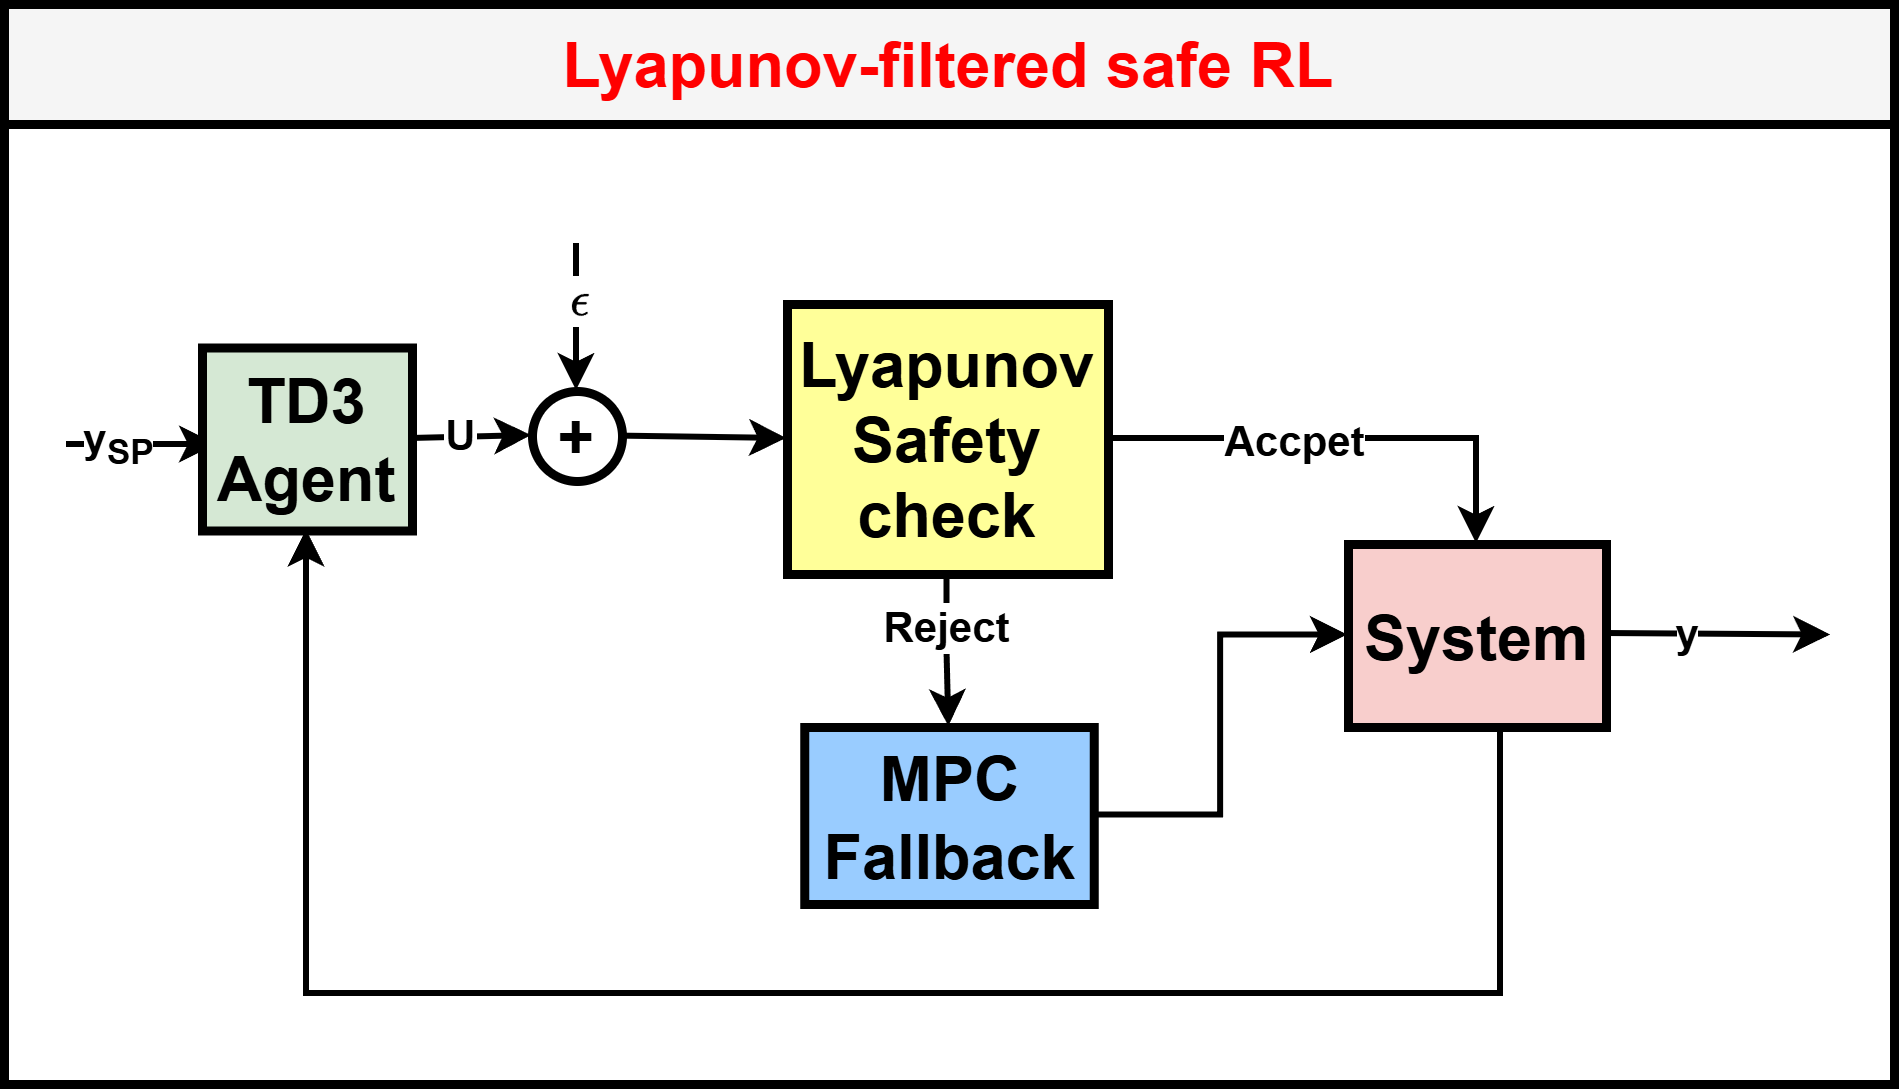
\includegraphics[width=\linewidth,height=0.16\textheight]{SafeRL.png}\\[-0.3em]
  \textbf{(c)}
\end{minipage}
\caption{Schematic figures for the three projects: (a) MPC-pretrained RL with offline imitation learning and online process interaction, (b) RL-assisted MPC, and (c) Lyapunov-filtered safe RL.}
\end{figure}

\CurrentStatus

The RL controller has been successfully developed and evaluated for both the polymerization reactor and Aspen Dynamics C2 splitter. The modified policy preserves the transient benefits of MPC-pretrained RL and reduces residual steady-state error relative to the baseline policy. For the C2 splitter, the controller improves performance across nominal operation, feed-flow fluctuations, and gradual feed ramps, while the online computation remains well below the available control interval. The results have been published in \emph{Industrial \& Engineering Chemistry Research}.

The RL-assisted MPC supervisor methodologies have produced strong polymer CSTR evidence. Scalar and structured model multipliers, weight and horizon tuning, residual correction, and the combined multi-agent supervisor all improve closed-loop reward relative to fixed MPC, with the combined supervisor giving the largest polymer improvement. For the Aspen Dynamics C2 splitter, closed-loop performance has also improved, but the final result comparison and packaging remain work in progress. These studies show that RL can assist MPC through interpretable supervisory adaptation while preserving the nominal MPC architecture rather than replacing it.

The Lyapunov-filtered safe RL methodology has been successfully demonstrated on the polymer CSTR. The controller combines TD3 action generation, target selection, Lyapunov-contraction certification, and MPC fallback within one supervisory structure. The distillation-column extension is currently in progress, with the same goal of allowing learned performance improvement while maintaining an explicit stability layer.

\bibliographystyle{unsrt}
\bibliography{research_summary_2026_draft}

\clearpage
\PosterSlides

\begin{center}
\centering
\begin{minipage}[t]{0.48\textwidth}
  \centering
  \includegraphics[width=\linewidth,keepaspectratio]{Slide1.PNG}
  \textbf{Slide 1}
\end{minipage}\hfill
\begin{minipage}[t]{0.48\textwidth}
  \centering
  \includegraphics[width=\linewidth,keepaspectratio]{Slide2.PNG}
  \textbf{Slide 2}
\end{minipage}

\begin{minipage}[t]{0.48\textwidth}
  \centering
  \includegraphics[width=\linewidth,keepaspectratio]{Slide3.PNG}
  \textbf{Slide 3}
\end{minipage}\hfill
\begin{minipage}[t]{0.48\textwidth}
  \centering
  \includegraphics[width=\linewidth,keepaspectratio]{Slide4.PNG}
  \textbf{Slide 4}
\end{minipage}

\begin{minipage}[t]{0.48\textwidth}
  \centering
  \includegraphics[width=\linewidth,keepaspectratio]{Slide5.PNG}
  \textbf{Slide 5}
\end{minipage}\hfill
\begin{minipage}[t]{0.48\textwidth}
  \centering
  \includegraphics[width=\linewidth,keepaspectratio]{Slide6.PNG}
  \textbf{Slide 6}
\end{minipage}
\end{center}

\end{document}
